\documentclass{article}
%%%%%%% PACKAGES %%%%%%%%
\usepackage[utf8]{inputenc}
\usepackage{graphicx}
\usepackage{geometry}
\geometry{a4paper, margin=1in}
\usepackage{hyperref}
\usepackage{titling}
\usepackage{caption}
\usepackage{subcaption}
\usepackage{float}
\hypersetup{
    colorlinks=true,
    linkcolor=blue,
    filecolor=magenta,      
    urlcolor=cyan,
}

\title{Assignment 2: Swarm Intelligence\\CS 451: Computational Intelligence}
\author{Ali Asghar Yousuf $\mid$ Muhammad Murtaza}
\date{\today}

\begin{document}

\maketitle

\section{Ant Colony Optimization}

\subsection*{\begin{center}
  Capacitated Vehicle Routing Problem
\end{center}}

\subsection{Problem Statement}
The Capacitated Vehicle Routing Problem (CVRP) is a variant of the Vehicle Routing Problem (VRP) in which each vehicle has a limited capacity. The problem is to find a set of routes for a fleet of vehicles to visit a set of customers, each with a demand, and return to the depot. The objective is to minimize the total distance traveled by all vehicles. The problem is NP-hard and is known to be computationally intractable for large instances. The problem is a special case of the Traveling Salesman Problem (TSP) in which the salesman has to visit a set of customers and return to the depot.

\subsection{Solution Approach}
We have used Ant Colony Optimization (ACO) to solve the Capacitated Vehicle Routing Problem. ACO is a metaheuristic optimization algorithm that is inspired by the behavior of real ants. The algorithm is based on the following steps:
\begin{enumerate}
  \item Initialization
  \item Ants' construction
  \item Pheromone update
  \item Termination
\end{enumerate}

\subsubsection{Initialization}
The first step is to initialize the parameters of the algorithm. The parameters are:
\begin{enumerate}
  \item $\alpha$ - Controls the importance of pheromone
  \item $\beta$ - Controls the importance of heuristic information
  \item $\gamma$ - Controls the importance of the capacity constraint
  \item $\texttt{numAnts}$ - Number of ants
  \item $\rho$ - Evaporation rate
  \item $\texttt{iteration}$ - Number of iterations
  \item $\texttt{capacity}$ - Capacity of each vehicle
  \item $\tau$ - Pheromone matrix
  \item $\eta$ - Heuristic matrix
  \item $\texttt{distances}$ - Distance matrix
  \item $\texttt{demand}$ - Demand matrix
\end{enumerate}

\subsubsection{Ants' construction}
In this step, the ants are initialized with random routes in the first iteration and in the next iterations they start constructing their routes. The ants are initialized at the depot and they move to the next node based on the following formula:
\begin{equation}
  P(i,j) = \frac{\tau_{i,j}^\alpha \eta_{i,j}^\beta}{\sum_{k \in \texttt{allowed}} \tau_{i,k}^\alpha \eta_{i,k}^\beta}
\end{equation}
where $\tau_{i,j}$ is the pheromone value of the edge between node $i$ and $j$, $\eta_{i,j}$ is the heuristic value of the edge between node $i$ and $j$, $\alpha$ and $\beta$ are the parameters of the algorithm, and $\texttt{allowed}$ is the set of nodes that are allowed to be visited by the ant. The ant moves to the next node based on the probability $P(i,j)$. The probability is calculated by taking the pheromone and heuristic values of the edges and then normalizing them. The ants move to the next node until they reach the depot or the capacity of the vehicle is exceeded. The ants then return to the depot and start constructing their routes again. This process is repeated for all the ants.

\subsubsection{Pheromone update}
In this step, the pheromone values of the edges are updated. The pheromone values are updated based on the following formula:
\begin{equation}
  \tau_{i,j} = (1 - \rho) \tau_{i,j} + \rho \tau_{i,j}^0
\end{equation}
where $\tau_{i,j}^0$ is the initial pheromone value of the edge between node $i$ and $j$, and $\rho$ is the evaporation rate of the algorithm. The pheromone values are updated after each iteration.

\subsubsection{Termination}
The algorithm terminates when the number of iterations reaches the maximum number of iterations. The best solution is the one with the least distance in all of the iterations.

\subsection{Optimal Solution}
After tweaking the parameters, and trying several different combinations we got the optimal values with the following parameters:
\begin{enumerate}
  \item $\alpha = 4$
  \item $\beta = 4$
  \item $\gamma = 0.5$
  \item $\texttt{numAnts} = 30$
\end{enumerate}

\subsubsection{A-n32-k5}
The minimum distance that we could achieve for this dataset was 807.475. The following is the route that we found:
\begin{figure}[H]
  \centering
  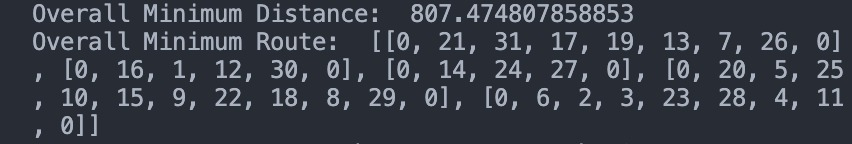
\includegraphics[width=1\linewidth]{images/min_dist_n32-k5.jpeg}
  \caption{Minimum Distance Route}
\end{figure}
Note: We forgot to plot this result, so the minimum distance for which we have a plot is 818.388
\begin{figure}[H]
  \centering
  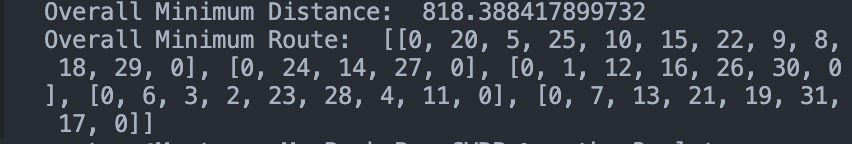
\includegraphics[width=1\linewidth]{images/min_dist2_n32-k5.jpeg}
  \caption{2nd Minimum Distance Route}
\end{figure}

\begin{figure}[H]
  \centering
  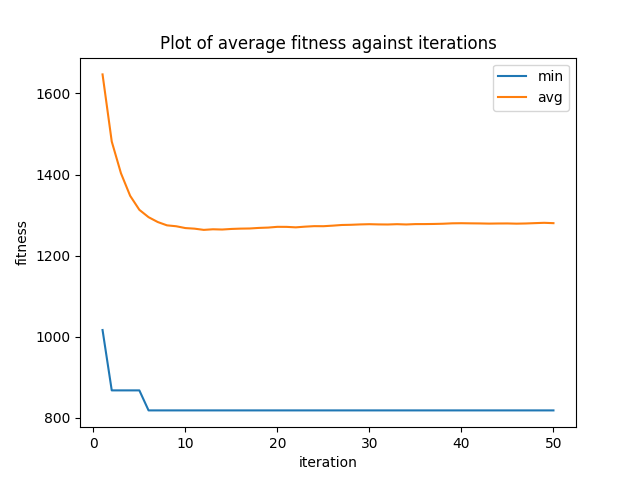
\includegraphics[width=1\linewidth]{images/min_n32-k5.png}
  \caption{2nd Minimum Distance Plot}
\end{figure}

\subsubsection{A-n44-k6}
The minimum distance that we could achieve for this dataset was 1118.325. The following is the route that we found:
\begin{figure}[H]
  \centering
  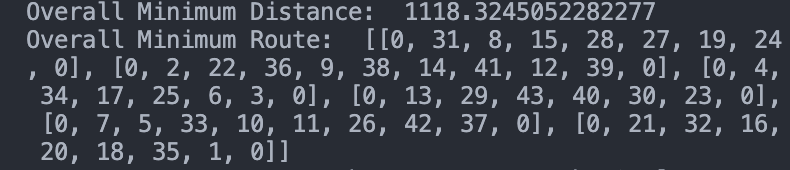
\includegraphics[width=1\linewidth]{images/min_dist_n44-k6.png}
  \caption{Minimum Distance Route}
\end{figure}
\begin{figure}[H]
  \centering
  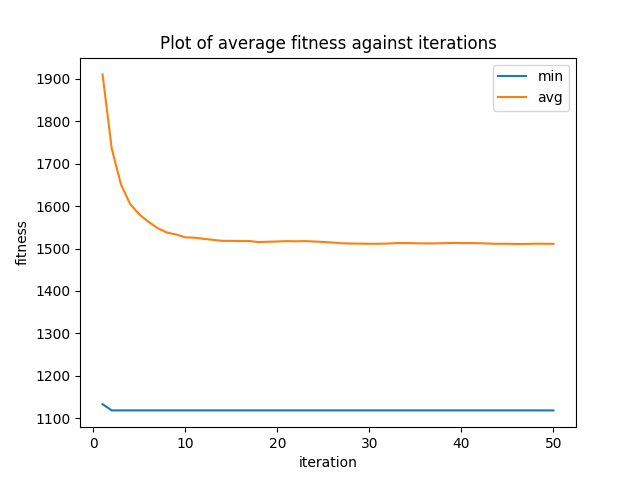
\includegraphics[width=1\linewidth]{images/min_n44-k6.png}
  \caption{Minimum Distance Plot}
\end{figure}

\subsubsection{A-n60-k9}
The minimum distance that we could achieve for this dataset was 1529.890. The following is the route that we found:
\begin{figure}[H]
  \centering
  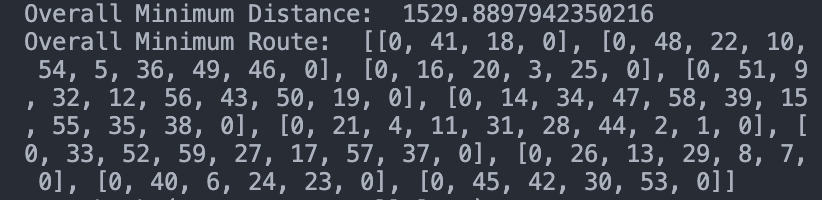
\includegraphics[width=1\linewidth]{images/min_dist_n60-k9.png}
  \caption{Minimum Distance Route}
\end{figure}

\begin{figure}[H]
  \centering
  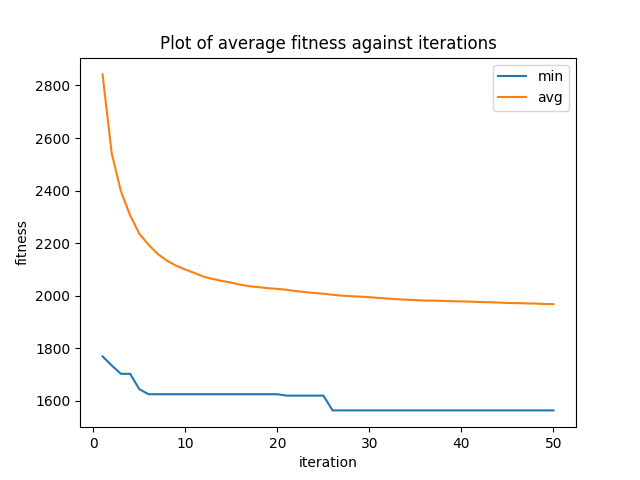
\includegraphics[width=1\linewidth]{images/min_n60-k9.png}
  \caption{Minimum Distance Plot}
\end{figure}

\subsubsection{A-n80-k10}
The minimum distance that we could achieve for this dataset was 2166.569. The following is the route that we found:
\begin{figure}[H]
  \centering
  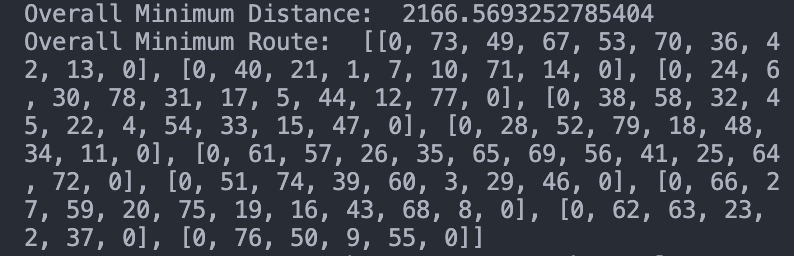
\includegraphics[width=1\linewidth]{images/min_dist_n80-k10.png}
  \caption{Minimum Distance Route}
\end{figure}

\begin{figure}[H]
  \centering
  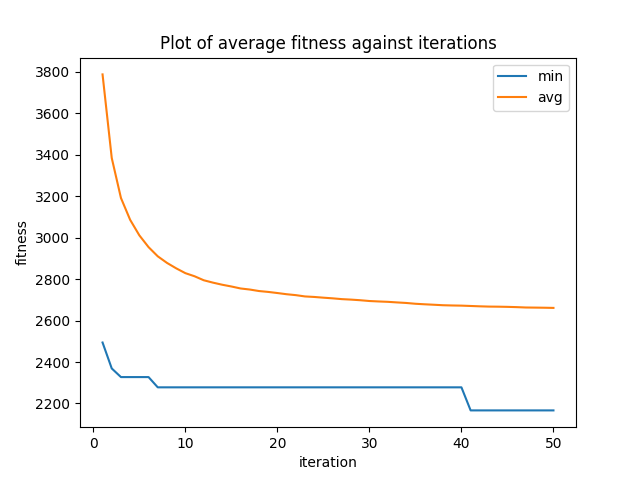
\includegraphics[width=1\linewidth]{images/min_n80-k10.png}
  \caption{Minimum Distance Plot}
\end{figure}

\subsection{Plot}
Plots of the best and average solution of Capacitated Vehicle Routing Problem using Ant Colony Optimization. The best solution is the one with the least distance. The average solution is the average of the distance of all the solutions in the population in each iteration.
\begin{figure}[H]
  \centering
  \textbf{Dataset A-n32-k5}
  \begin{subfigure}{.5\textwidth}
    \centering
    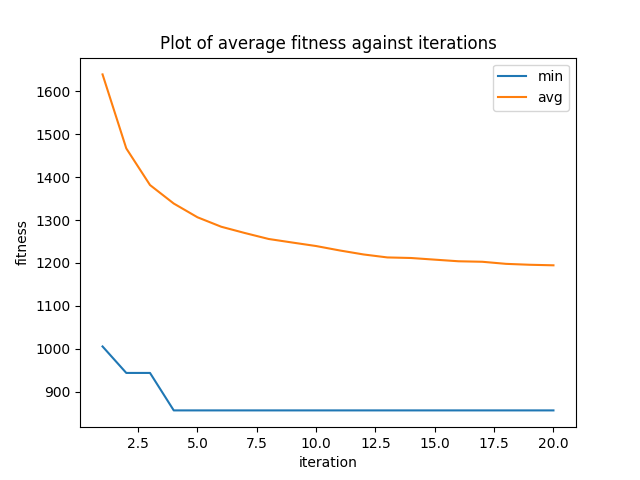
\includegraphics[width=1\linewidth]{images/n32-k5_20.png}
    \caption{ACO with 20 iterations}
    \label{fig:n32-k5_20}
  \end{subfigure}%
  \begin{subfigure}{.5\textwidth}
    \centering
    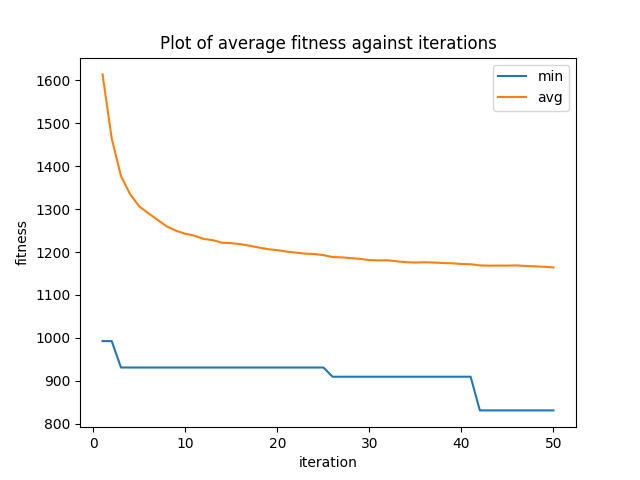
\includegraphics[width=1\linewidth]{images/n32-k5_50.png}
    \caption{ACO with 50 iterations}
    \label{fig:n32-k5_50}
  \end{subfigure}
  \caption{Note: Fitness is the distance}
  \label{fig:n32-k5}
\end{figure}

\begin{figure}[H]
  \centering
  \textbf{Dataset A-n44-k6}
  \begin{subfigure}{.5\textwidth}
    \centering
    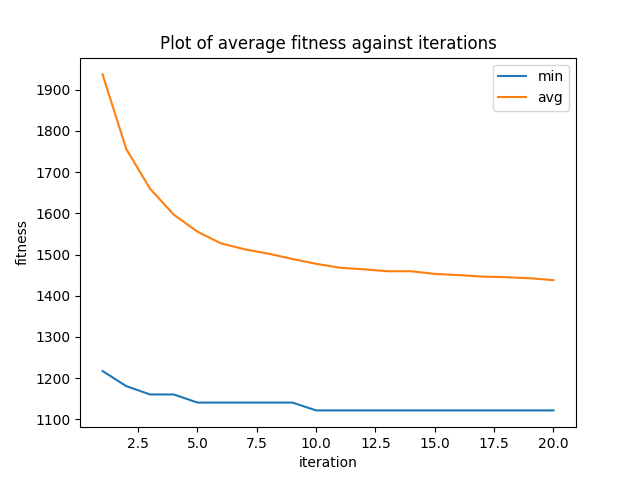
\includegraphics[width=1\linewidth]{images/n44-k6_20.png}
    \caption{ACO with 20 iterations}
    \label{fig:n44-k6_20}
  \end{subfigure}%
  \begin{subfigure}{.5\textwidth}
    \centering
    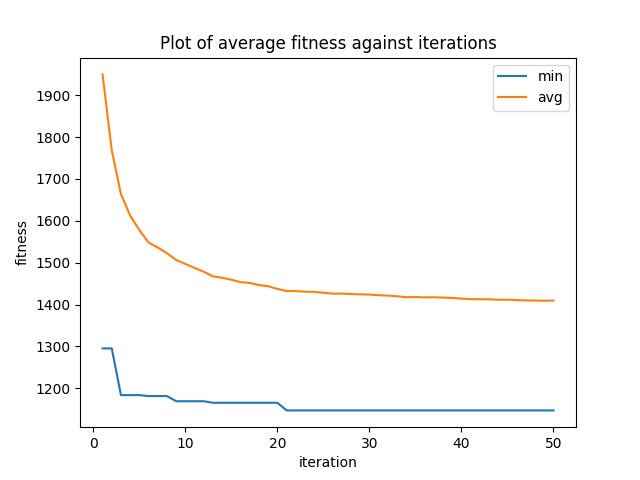
\includegraphics[width=1\linewidth]{images/n44-k6_50.png}
    \caption{ACO with 50 iterations}
    \label{fig:n44-k6_50}
  \end{subfigure}
  \caption{Note: Fitness is the distance}
  \label{fig:n44-k6}
\end{figure}

\begin{figure}[H]
  \centering
  \textbf{Dataset A-n60-k9}
  \begin{subfigure}{.5\textwidth}
    \centering
    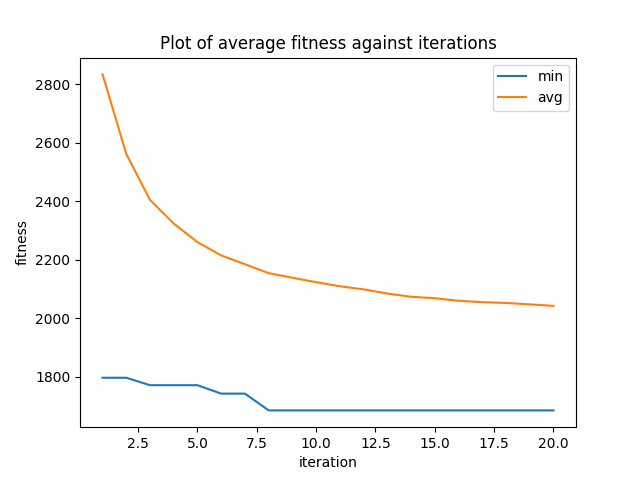
\includegraphics[width=1\linewidth]{images/n60-k9_20.png}
    \caption{ACO with 20 iterations}
    \label{fig:n60-k9_20}
  \end{subfigure}%
  \begin{subfigure}{.5\textwidth}
    \centering
    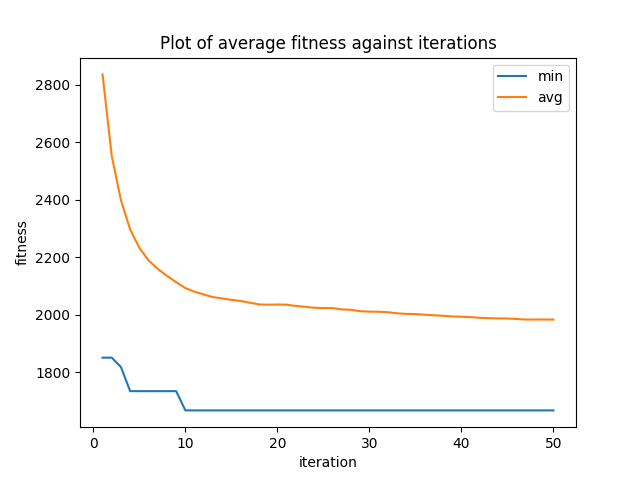
\includegraphics[width=1\linewidth]{images/n60-k9_50.png}
    \caption{ACO with 50 iterations}
    \label{fig:n60-k9_50}
  \end{subfigure}
  \caption{Note: Fitness is the distance}
  \label{fig:60-k9}
\end{figure}

\begin{figure}[H]
  \centering
  \textbf{Dataset A-n80-k10}
  \begin{subfigure}{.5\textwidth}
    \centering
    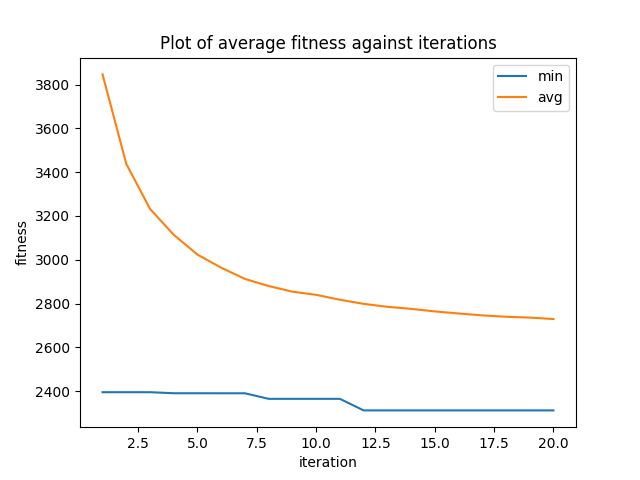
\includegraphics[width=1\linewidth]{images/n80-k10_20.png}
    \caption{ACO with 20 iterations}
    \label{fig:n80-k10_20}
  \end{subfigure}%
  \begin{subfigure}{.5\textwidth}
    \centering
    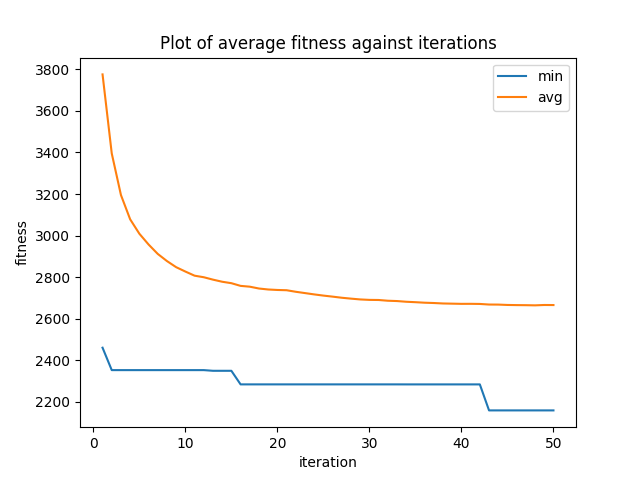
\includegraphics[width=1\linewidth]{images/n80-k10_50.png}
    \caption{ACO with 50 iterations}
    \label{fig:n80-k10_50}
  \end{subfigure}
  \caption{Note: Fitness is the distance}
  \label{fig:n80-k10}
\end{figure}

\section{Visualizing Swarms}

\subsection*{\begin{center}
  Visualizing Smoke Particle from Car Exhaust System
\end{center}}

\textbf{Given the current climate change events, it is important to create awareness of our daily carbon footprint, so we have made this smoke simulator that will aware people of how a car can damage our atmosphere, while at the same time we can represent particle system with it.}
\\~\\
Particle System is a collection of many minute particles that together represent a fuzzy object. Here we have a smoke particles that together will represent smoke from car exhaust system. 

\begin{figure}[H]
  \centering
    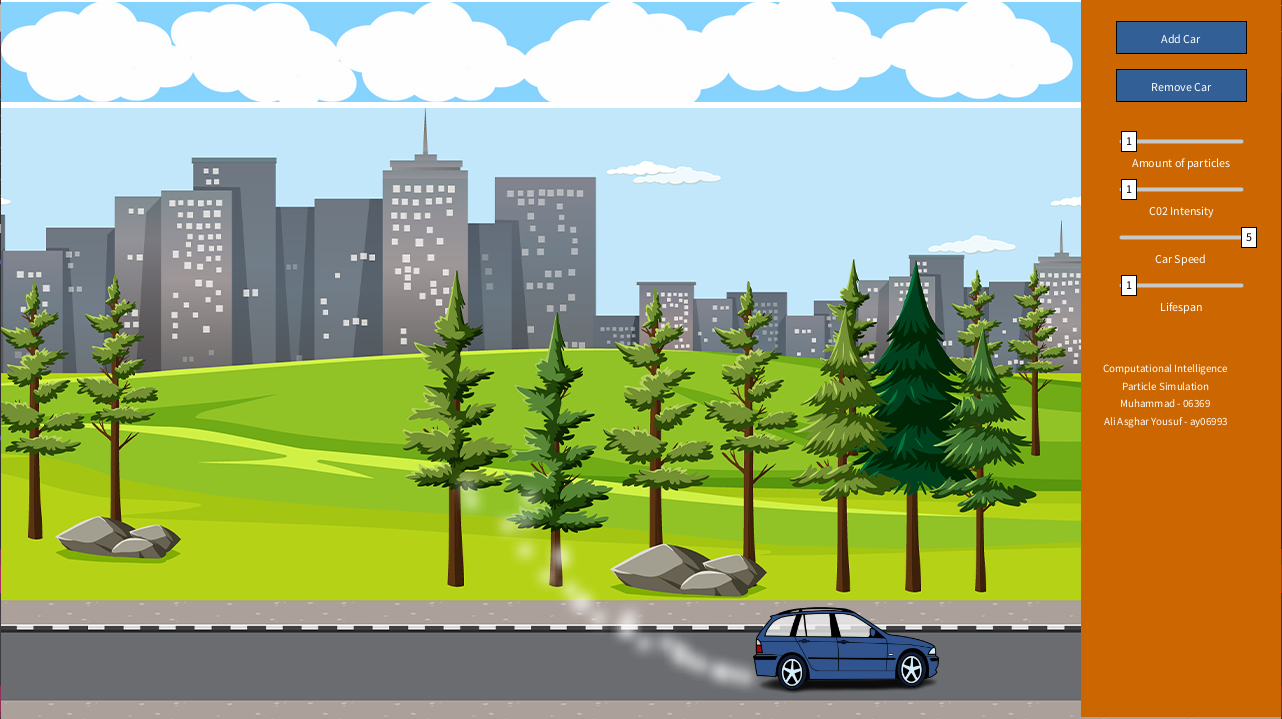
\includegraphics[width=1\linewidth]{images/simulator.png}
    \caption{Car Exhaust Smoke Simulator}
\end{figure}

\textbf{First we will classify all the attributes of a particle system}
\\
\begin{itemize}
  \item Position: Each particle has a given position on the screen with 'x' and 'y' coordinate.
  \item Velocity: Each particle has a randomly generated velocity which is constant. 
  \item Lifetime: Life of a particle can be changed in this system. When a life of particle ends, it dies from the system. 
  \item Color: Initially it is white, if the CO2 intensity increases, it becomes black.
  \item Shape: The particle has round shape.
  \item Size: 16 pixels.
\end{itemize}

\textbf{Each of the following phases of particles has been implemented in this system}
\begin{itemize}
    \item Particle Lifespan
    \begin{itemize}
      \item{Each particle is generated randomly in each iteration}
      \item{Particles moves upwards towards the sky.}
      \item{Particle is rendered on the screen on each given position}
      \item{Particle then reaches extinction phase when it dies from the system}
    \end{itemize}
    \item Particle Generation
    \begin{itemize}
      \item{Particle is generated in each iteration of the system randomly. We can control particle generation by increasing or decreasing its chances of generation in the given system.}
    \end{itemize}
    \item Particle Dynamics
    \begin{itemize}
      \item{The particle has a position vector and it is moved by adding the corresponding velocity vector to it.}
      \item{The particle has a zero acceleration and its velocity is kept constant. However acceleration can be added to velocity.}
    \end{itemize}
    \item Extinction
\end{itemize}

\textbf{The video of the simulation can be seen here: }
\href{https://www.youtube.com/watch?v=BU9WsN1110Y}{https://www.youtube.com/watch?v=BU9WsN1110Y}


\end{document}
